\begin{flushright} {\tiny {\color{gray} python\_codes/fieldstone\_128/text.tex}} \end{flushright}

\lstinputlisting[language=bash,basicstyle=\small]{python_codes/fieldstone_128/keywords}

\begin{center}
\fbox{\textbf{\huge \color{teal} P}}
Codes at \url{https://github.com/cedrict/fieldstone/tree/master/python_codes/fieldstone_128}
\end{center}

\par\noindent\rule{\textwidth}{0.4pt}

%%%%%%%%%%%%%%%%%%%%%%%%%%%%%%%%%%%%%%%%%%%%%%%%%%%%%%%%%%%%%%%%%%%%%%%%%%%%%%%%%%%%%%%%%%%%%%

Following chapter 10 of Guy Simpson's book \cite{simp17} the equations
governing the evolution of the fluid pressure and fluid flow velocities are\footnote{I have slightly changed the notations.}
\begin{eqnarray}
\varphi \beta \frac{\partial p}{\partial t} &=& -\vec\nabla \cdot \vec \upnu + H \label{eq:128:a}\\
\vec\upnu &=& -\frac{K}{\eta_f} \left(\vec\nabla p - \rho_f g \vec{e}_z \right) \label{eq:128:b}
\end{eqnarray}
where
\begin{itemize}
\item $p$ is the fluid pressure, 
\item $\vec\upnu$ is the fluid velocity vector, 
\item $\varphi$ is the porosity, 
\item $\beta$ is the bulk compressibility (\si{\per\pascal}), 
\item $K$ is the permeability (\si{\square\meter}), 
\item $\eta_f$ is the fluid viscosity (\si{\pascal\second}), 
\item $\rho_f$ is the water density (\si{\kg\per\cubic\meter}), 
\item $g$ is acceleration due to gravity (\si{\meter\per\square\second}), 
\item $\vec{e}$ is a unit vector oriented in the vertical direction, 
\item $H$ accounts for any fluid pressure sources or sinks (e.g., due to devolatilization reactions)
\end{itemize}
Introducing the excess pore fluid pressure defined as the pressure in excess of the hydrostatic pressure 
(i.e., $p_e = p-p_h$ where $p_h = \rho_f g (L_z-z)$) and 
substituting \eqref{eq:128:b} into \eqref{eq:128:a} lead to a single parabolic equation for
the excess fluid pressure as follows:
\begin{equation}
\varphi \beta  \frac{\partial p_e}{\partial t}
=
\vec\nabla \cdot \left( \frac{K}{\eta_f} \vec\nabla p_e  \right) + H
\end{equation}
Note that once the excess pressure is computed one can recover the fluid velocity via $\vec\upnu=-\frac{K}{\eta_f} \vec\nabla p_e$. 

%--------------------------------------------------------------------------------------
\subsection*{Fluid Flow Around a Fault (experiment=2)}

%from simpson book
A porous crust with an initially uniform and isotropic permeability has an
overpressure that increases linearly with depth. At $t=0$ a dipping, high permeability fault zone is
suddenly introduced into the crust.
The transient evolution of the excess pore pressure is governed by
\begin{equation}
\varphi \beta  \frac{\partial p_e}{\partial t}
=
\vec\nabla \cdot \left( \frac{K(x,y)}{\eta_f} \vec\nabla p_e  \right) 
\end{equation}
subject to the boundary conditions as specified in the following figure:
\begin{center}
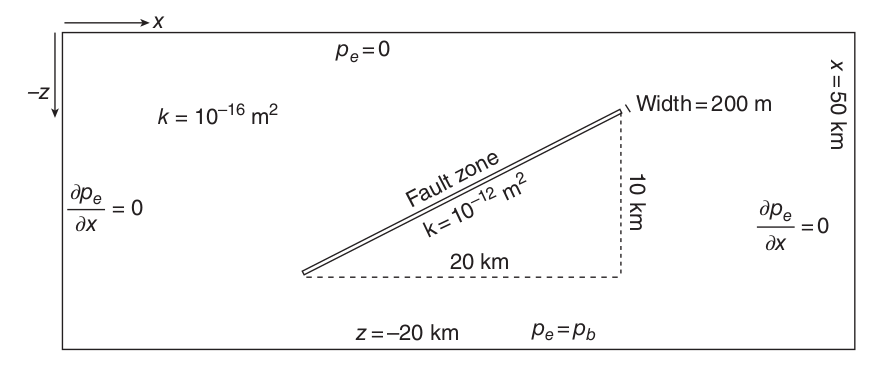
\includegraphics[width=11cm]{python_codes/fieldstone_128/images/simpson1}\\
{\captionfont Taken from \cite{simp17}. Setup for model of fluid flow around a high permeability fault zone.}
\end{center}

In the book the problem was solved with a total of 5248 triangles, 
a time step of 0.1 years, and the following physical parameters:
$K_{crust}=10^{-16}~\si{\square\meter}$ , 
$K_{fault}=10^{-12}~\si{\square\meter}$ , 
$\eta_f  = \SI{1.33e-4}{\pascal\second}$, 
$\beta=\SI{1e-10}{\per\pascal}$, and $\varphi=0.1$. 
The results, after an approximately steady situation has been achieved (after 10 years), show how the fluid overpressure
and fluid flow vectors in the crust are strongly perturbed by the presence of the high permeability
fault zone. Fluid is focused toward the base of the fault, while it diverges away from its upper tip.
\begin{center}
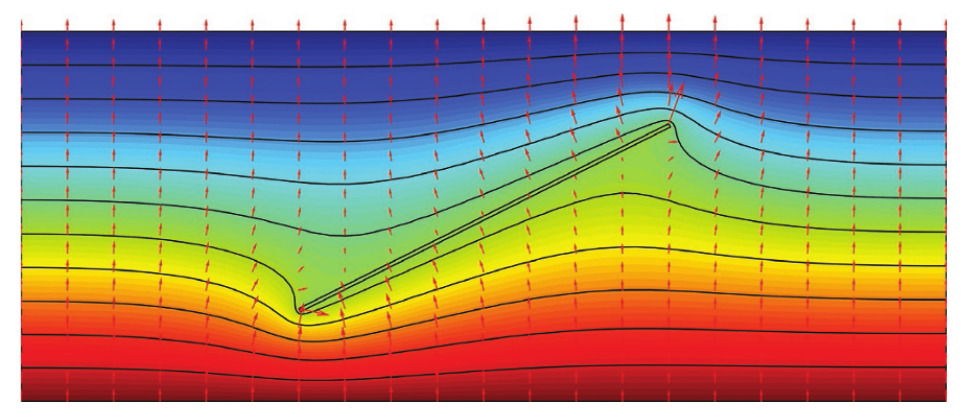
\includegraphics[width=12cm]{python_codes/fieldstone_128/images/simpson2}\\
{\captionfont Taken from \cite{simp17}. Excess fluid pressure and flow vectors in the crust 
(with a uniform permeability of $\SI{1e-16}{\per\square\meter}$) 10 years after
introduction of a high permeability ($\SI{1e-12}{\per\square\meter}$) fault zone.}
\end{center}

The matlab code in the book relies on a bespoke mesh of linear triangles. Unfortunately the 
mesh is stored in a {\tt .mat} format which is very inconvenient. In this \stone we rely on 
linear quadrilaterals ($Q_1$) instead. 

In what follows we use a $500\times 200$ mesh. Because of the geometry of the fault and the fact that we rely on 
a regular mesh, the fault is then represented as follows in the model:

\begin{center}
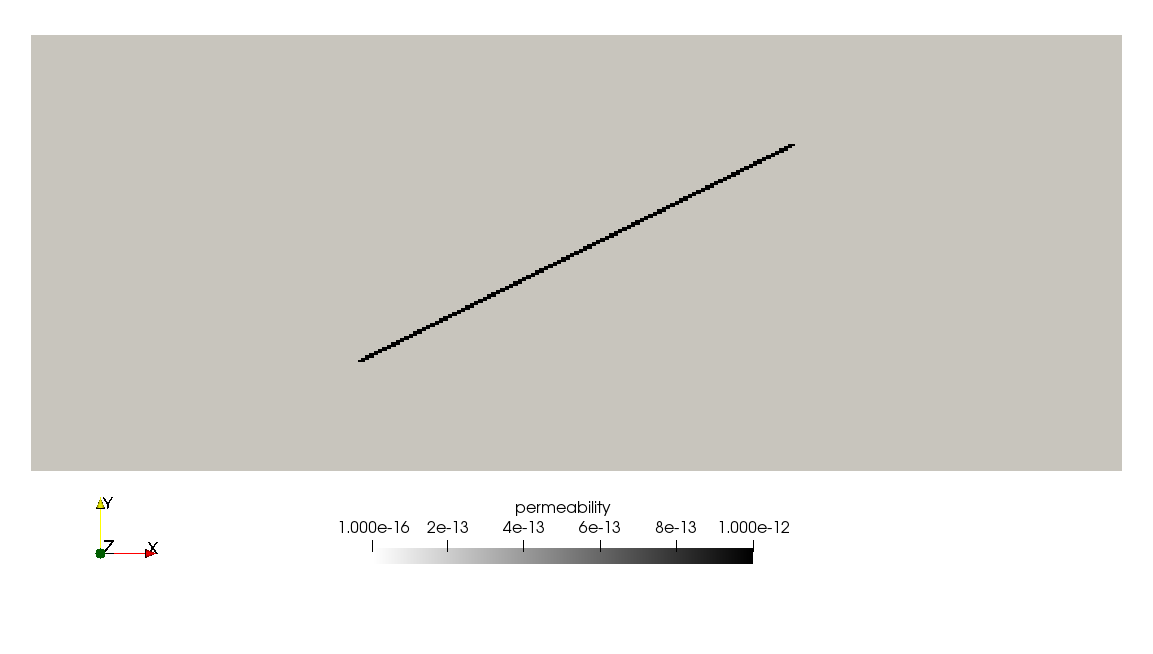
\includegraphics[width=9cm]{python_codes/fieldstone_128/results/experiment2/K}
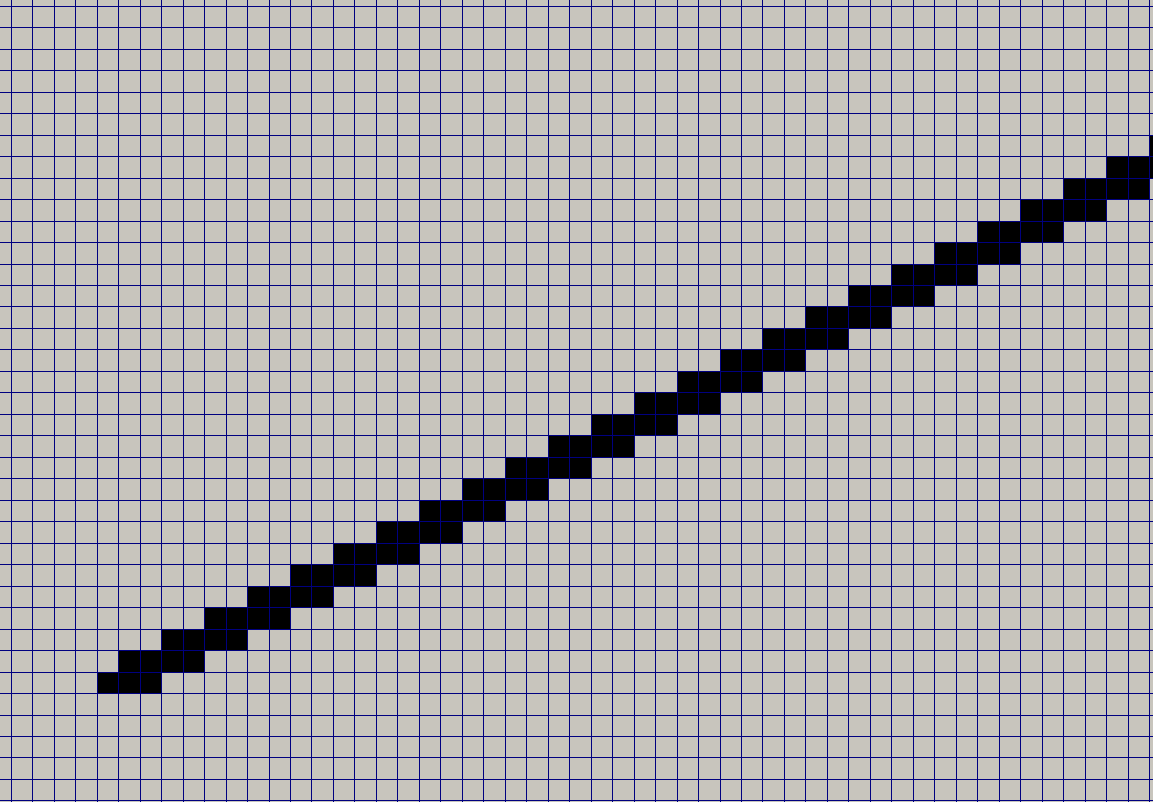
\includegraphics[width=7cm]{python_codes/fieldstone_128/results/experiment2/K_zoom}\\
{\captionfont Permeability on 500x200 mesh.}
\end{center}

The rest of the code is rather straight forward since it is a diffusion equation
(see for instance \stone 03). We carry out 100 timesteps of $\delta t=0.1~\si{\year}$ each, 
which is indeed enough time to reach a steady state. The recovered pressure and velocity fields 
are similar to those in the book but since the book's figure does not showcase a colorscale
we cannot quantitatively compare\footnote{Run code with Matlab?}.
The velocitiy field is essentially a scaled pressure gradient and we compute it in the middle 
of each element for simplicity. The code computes the root mean square velocity and 
the average pressure over the domain.

\begin{center}
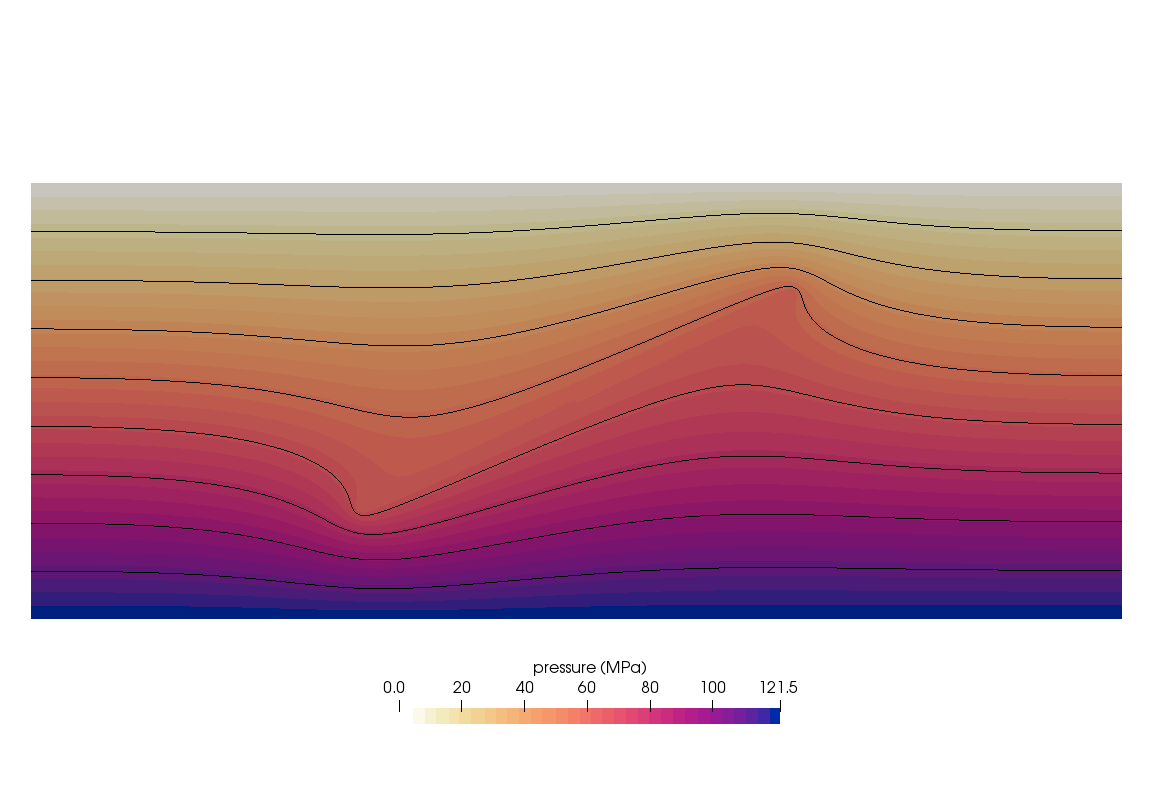
\includegraphics[width=8cm]{python_codes/fieldstone_128/results/experiment2/press}
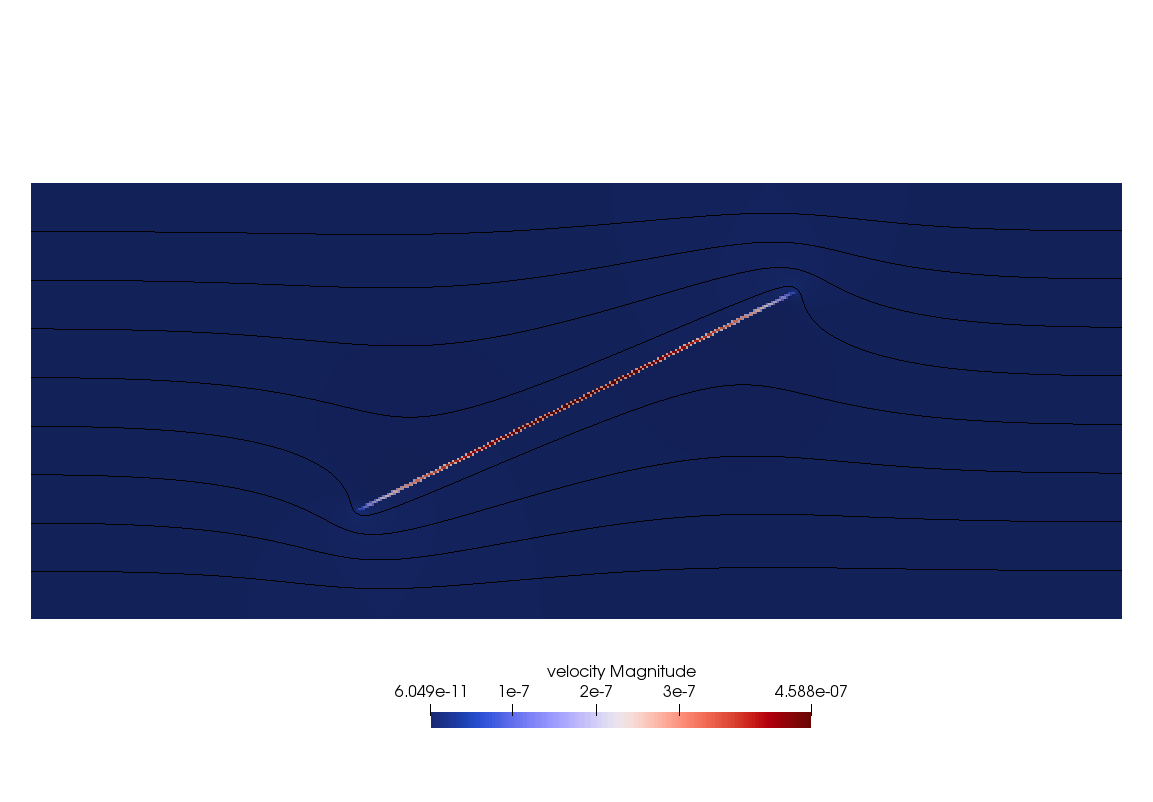
\includegraphics[width=8cm]{python_codes/fieldstone_128/results/experiment2/vel}\\
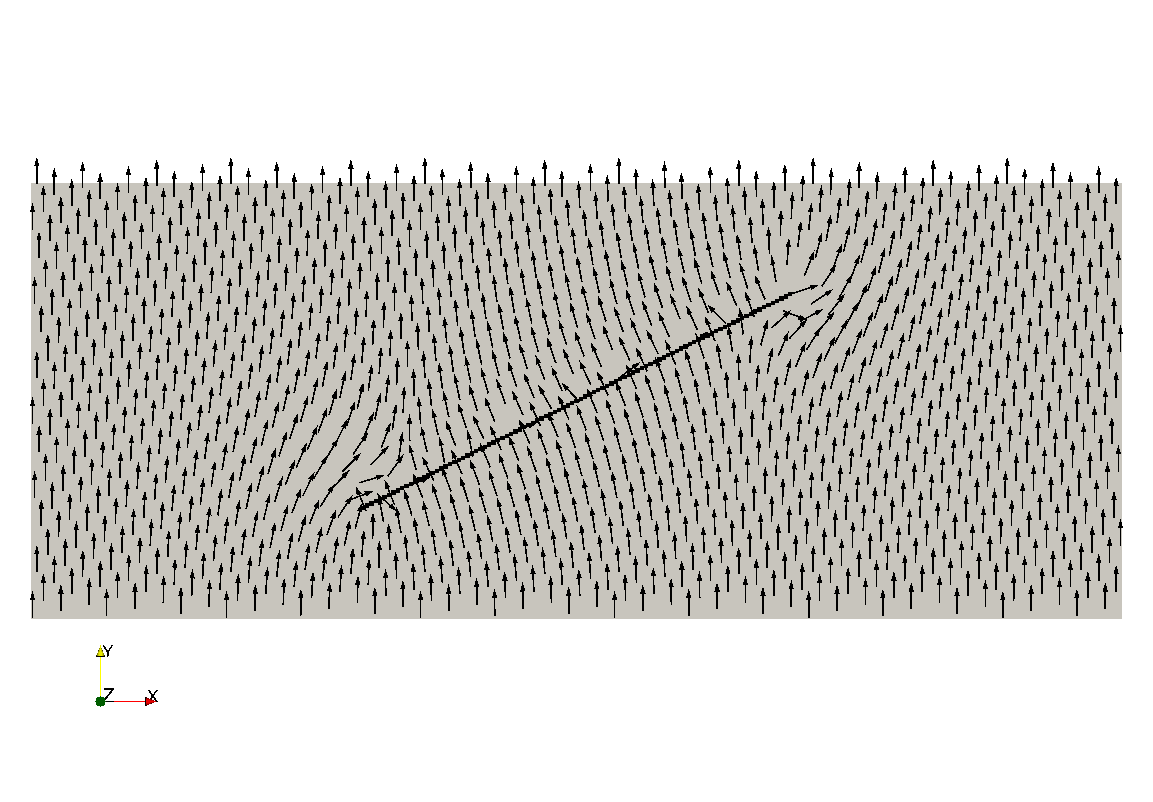
\includegraphics[width=12cm]{python_codes/fieldstone_128/results/experiment2/flow}\\
{\captionfont Pressure and velocity field at $t=10~\si{\year}$. Note that there is a very large 
difference in velocity magnitude between the crust and the fault. The flow arrows are actually 
obtained by normalising the velocity vector to one in each element.}
\end{center}

\begin{center}
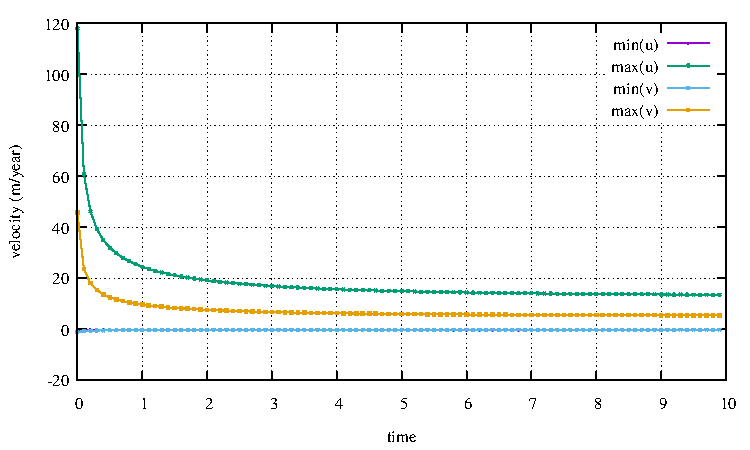
\includegraphics[width=8cm]{python_codes/fieldstone_128/results/experiment2/velocity}
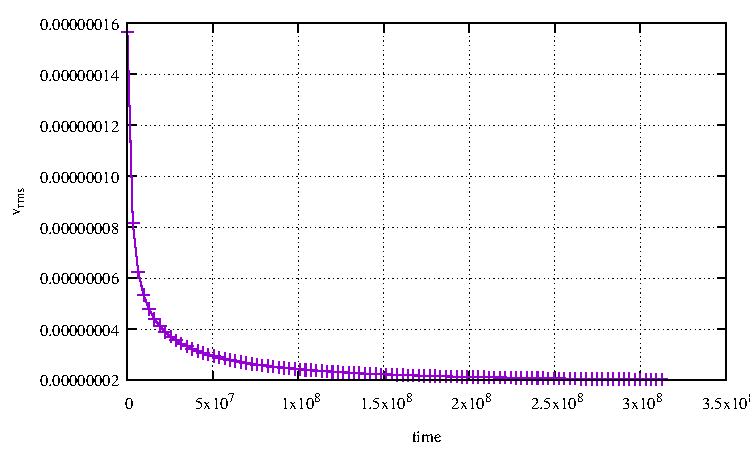
\includegraphics[width=8cm]{python_codes/fieldstone_128/results/experiment2/vrms}\\
{\captionfont Velocity statistics. Pressure stats and average plots are not interesting
so not shown.}
\end{center}


%--------------------------------------------------------------------------------------
\subsection*{Fluid Flow Around a circular inclusion (experiment=1)}

Same setup as experiment 2, but the fault has now been replaced by a circular inclusion 
placed in the middle of the domain and of radius 5~\si{\km}.

\begin{center}
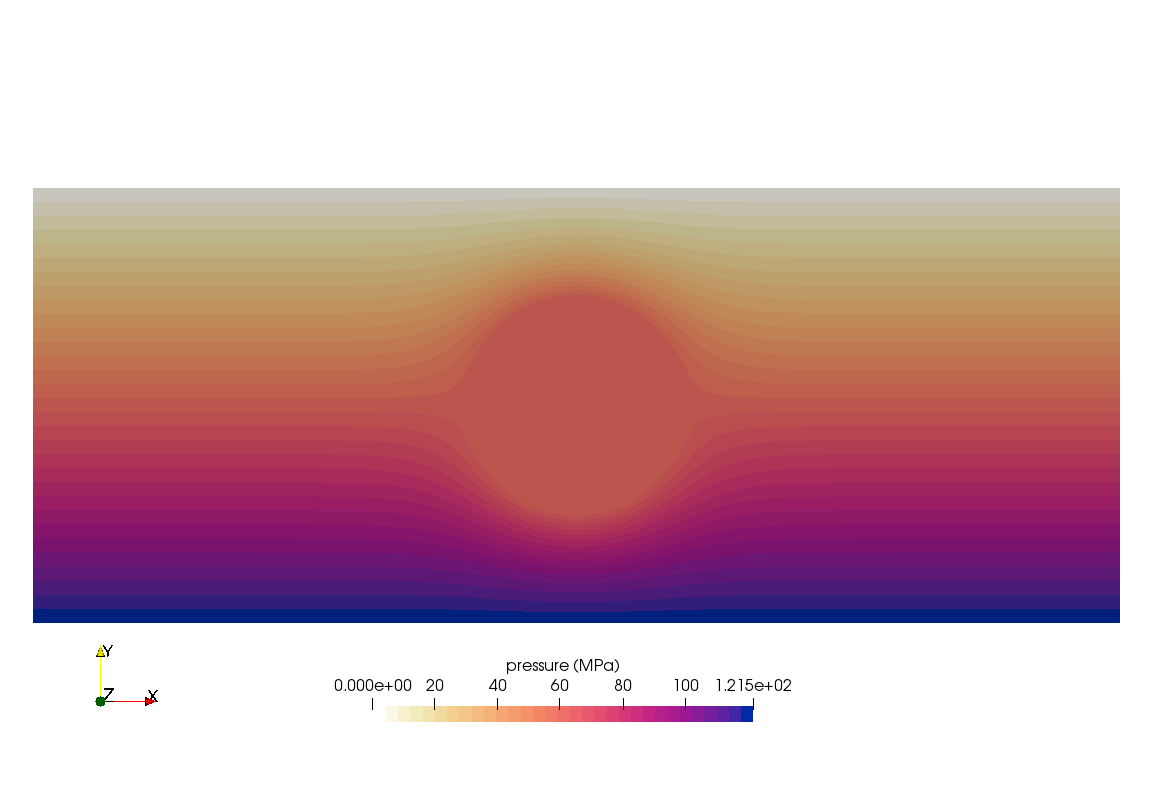
\includegraphics[width=8cm]{python_codes/fieldstone_128/results/experiment1/press}
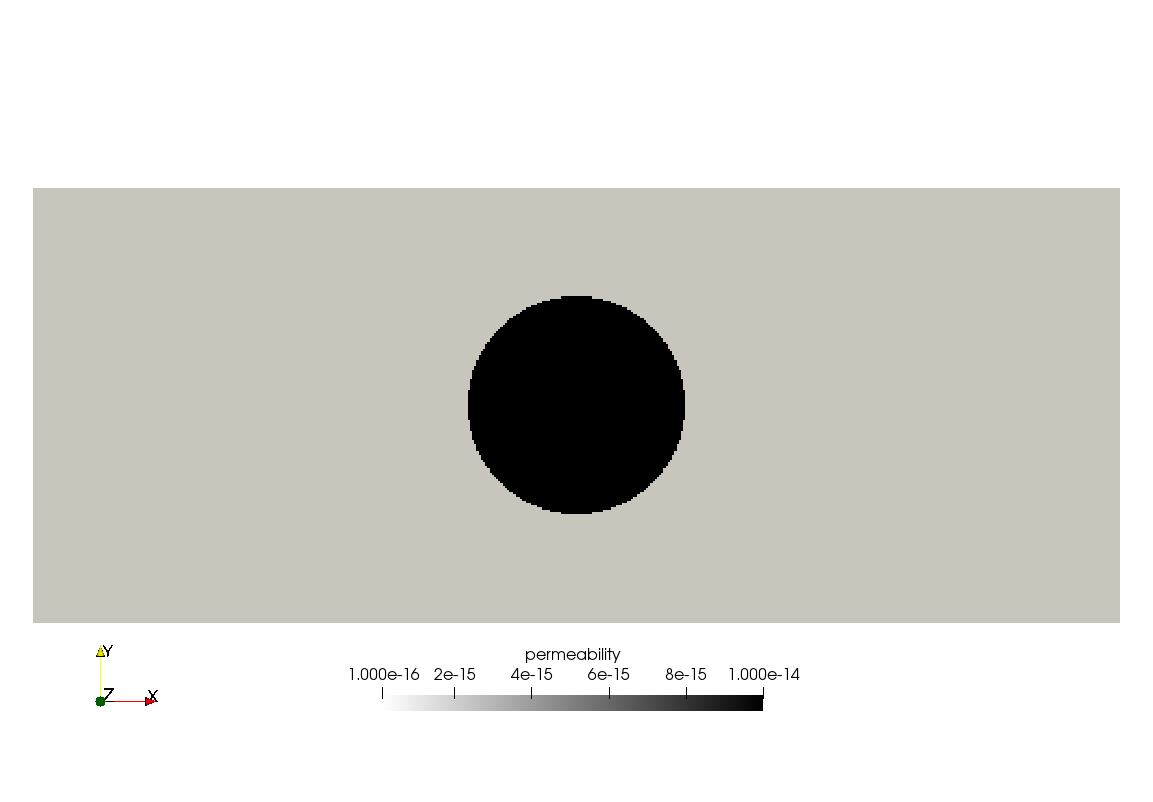
\includegraphics[width=8cm]{python_codes/fieldstone_128/results/experiment1/K}\\
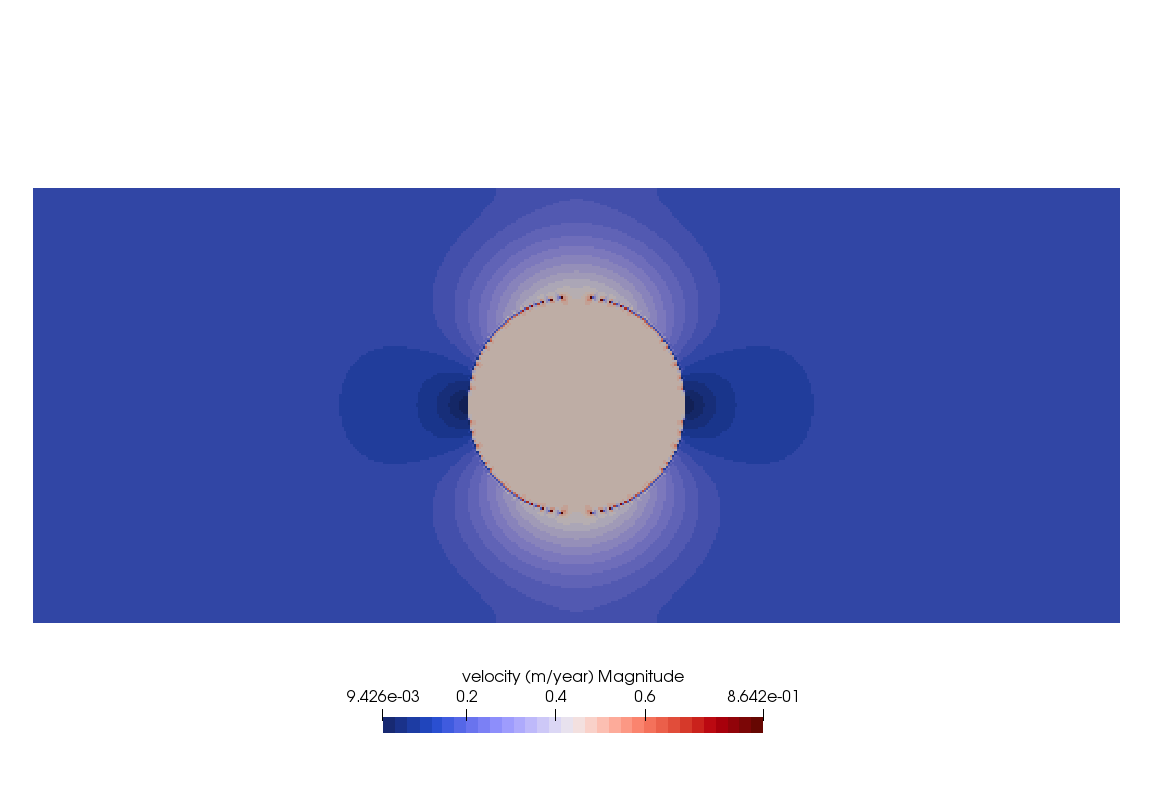
\includegraphics[width=8cm]{python_codes/fieldstone_128/results/experiment1/vel}
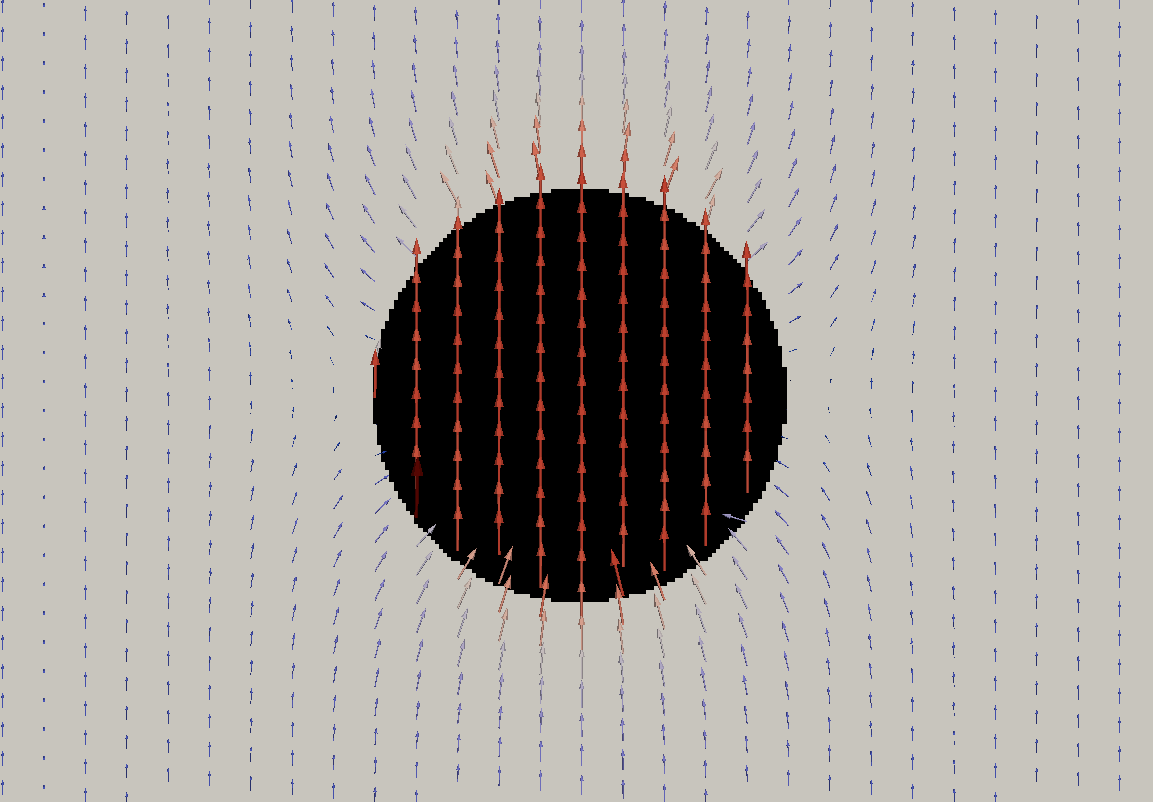
\includegraphics[width=8cm]{python_codes/fieldstone_128/results/experiment1/vel2}\\
\end{center}


%--------------------------------------------------------------------------------------
\subsection*{Fluid Flow in a  (experiment=3)}

All parameters are identical to experiment 2. However I have placed
111 random seeds in the domain and computed the voronoi diagram of these 
as projected onto the elements:

\begin{center}

\includegraphics[width=8cm]{python_codes/fieldstone_128/results/experiment3/cells}

\includegraphics[width=8cm]{python_codes/fieldstone_128/results/experiment3/cells_zoom}
\end{center}

Each Voronoi cell is then 
attributed a random permeability between $10^{-14}$ and $10^{-16}$, 
using the algorithm documented in \stone~125.
Two bands of thickness $L_y/6$ with constant permeability $10^{-15}$ are 
prescribed at the top and bottom of the domain.
Simulations are run until steady state is reached. 

\begin{center}
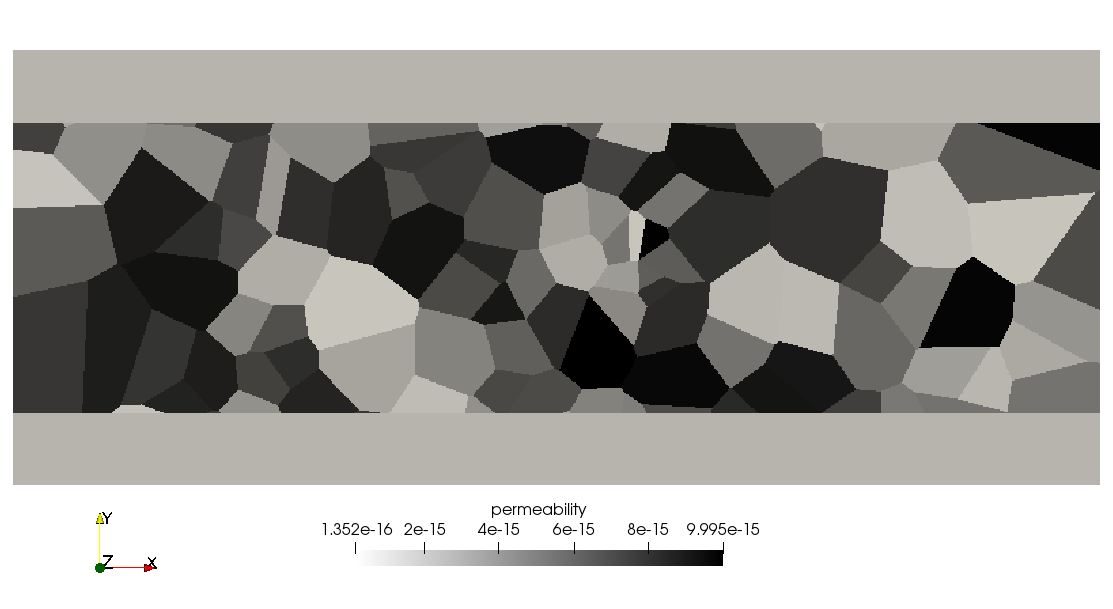
\includegraphics[width=13cm]{python_codes/fieldstone_128/results/experiment3/K}\\
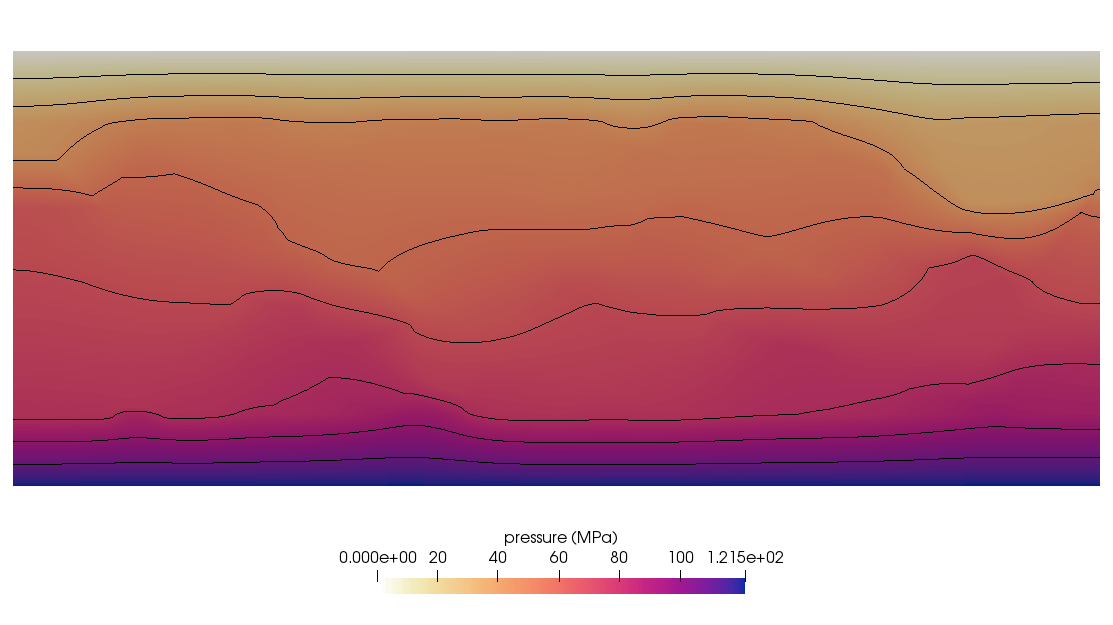
\includegraphics[width=13cm]{python_codes/fieldstone_128/results/experiment3/press}\\
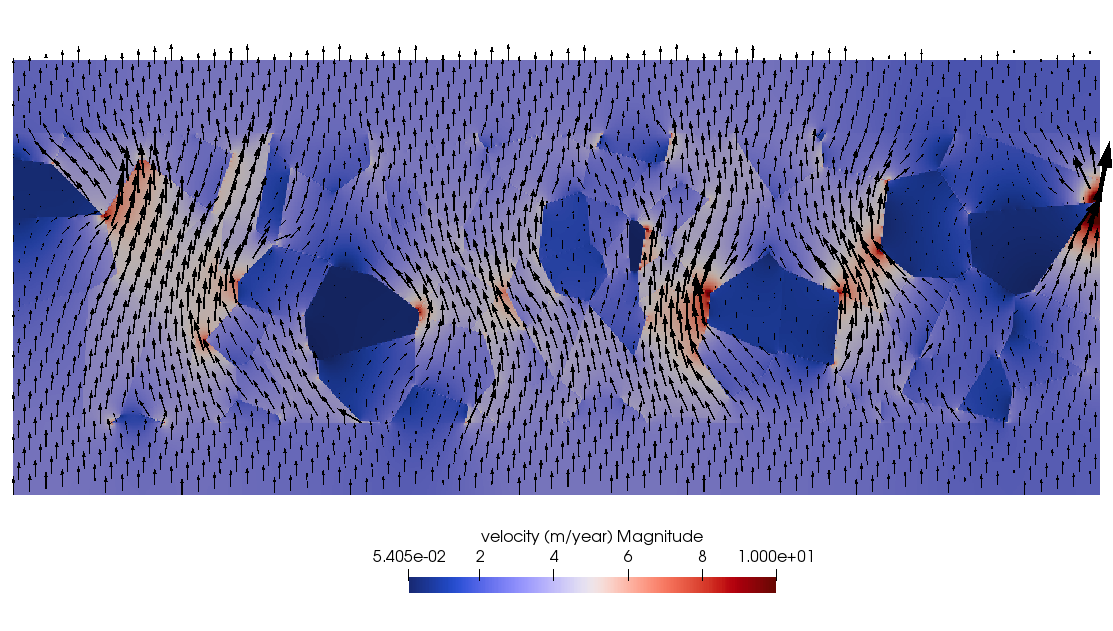
\includegraphics[width=13cm]{python_codes/fieldstone_128/results/experiment3/vel}\\
{\captionfont Run on 800x320 mesh. This could easily be increased.} 
\end{center}

Remark: this setup as it is now makes no sense. However, it could be scaled down to a few meters or
centimeters. Pressure boundary conditions and permeability values can also be adapted.
Three-dimensional simulations could equally easily be run, albeit with a much higher
computational cost. 
Obviously the number of 'grains', their position, their permeability, etc ... can be 
changed too.


